\documentclass[11pt,a4paper]{ctexart}

\usepackage{amsmath,amssymb,bm}
\usepackage{geometry}
\usepackage{enumitem}
\usepackage{fancyhdr}
\usepackage{lastpage}
\usepackage{xcolor}
\usepackage{tcolorbox}
\usepackage{tikz}
\usepackage{titlesec}
\usepackage{microtype}
\usepackage{cases}
\usetikzlibrary{arrows.meta,calc}

\geometry{left=2.15cm,right=2.15cm,top=2.0cm,bottom=2.0cm}
\setlength{\parindent}{2em}
\setlength{\parskip}{0.25em}
\linespread{1.12}

\definecolor{mainblue}{RGB}{39,91,150}
\definecolor{lightblue}{RGB}{232,241,252}
\definecolor{darkgray}{RGB}{65,65,65}
\definecolor{lightgray}{RGB}{245,246,248}

\titleformat{\section}{\large\bfseries\color{mainblue}}{}{0em}{}[\titlerule]
\titleformat{\subsection}{\normalsize\bfseries\color{darkgray}}{}{0em}{}
\titlespacing*{\section}{0pt}{0.9em}{0.45em}
\titlespacing*{\subsection}{0pt}{0.65em}{0.25em}

\setlist[enumerate]{leftmargin=2.2em,itemsep=0.25em,topsep=0.25em}
\setlist[itemize]{leftmargin=2.0em,itemsep=0.2em,topsep=0.2em}

\pagestyle{fancy}
\fancyhf{}
\lhead{\small 格物助航｜每日一练}
\rhead{\small 2026.6.12}
\cfoot{\small 第 \thepage\ 页 / 共 \pageref{LastPage} 页}
\renewcommand{\headrulewidth}{0.4pt}

\newtcolorbox{problemBox}{
  colback=lightblue,
  colframe=mainblue,
  arc=2mm,
  boxrule=0.7pt,
  left=1.0em,
  right=1.0em,
  top=0.8em,
  bottom=0.8em,
  before skip=0.6em,
  after skip=0.8em
}

\newtcolorbox{tipBox}{
  colback=lightgray,
  colframe=darkgray,
  arc=1.5mm,
  boxrule=0.5pt,
  left=0.9em,
  right=0.9em,
  top=0.6em,
  bottom=0.6em,
  before skip=0.5em,
  after skip=0.5em
}

\newcommand{\dd}{\mathrm{d}}
\newcommand{\ii}{\bm{i}}
\newcommand{\jj}{\bm{j}}

\begin{document}

\begin{center}
  {\Large\bfseries\color{mainblue} 格物助航｜每日一练}\par
  \vspace{0.25em}
  {\large 力学第七章：刚体力学}\par
  \vspace{0.35em}
  {\small 2026年6月12日}\par
  \vspace{0.35em}
  {\small 编写：谢奕明}
\end{center}

\vspace{-0.3em}

\section*{解题技巧和思路}
\begin{tipBox}
处理刚体转动的问题时，可按以下步骤进行：
\begin{enumerate}
\item \textit{明确研究对象，标出所有力及其作用点（对于摩擦力则需要根据相对运动趋势确定摩擦力的方向），明确初始条件对应的滚动是纯滚动还是边滑动边滚动，据此确定摩擦力是静摩擦力还是滑动摩擦力；}
\item \textit{列出平动和转动的动力学方程，确定守恒量并对应列出能量、动量、角动量守恒方程，注意转动方程选取的参考点；}
\item \textit{列出纯滚动的运动学约束条件，将角加速度与质心加速度关联；}
\item \textit{联立方程解出各力随位置的变化；}
\item \textit{根据题目求解出最终所需的物理量}
\end{enumerate}
（如果是纯滚动，则可以多列一个接触点速度为零的约束方程，但没有$f  = \mu N$这一方程；如果是边滑动边滚动，那么少了一个约束方程，但多了$f = \mu N$这一方程）
\end{tipBox}

\section*{习题再现}
\begin{problemBox}
\noindent\textbf{题目}\quad
如图所示，质量为$m$，半径为$r$的小球从半径为$R$的固定圆柱面顶端受微小扰动后滚下。为保证在$\theta \leq 45^\circ$的范围内小球作纯滚动，试求静摩擦因数$\mu$的最小值。

\vspace{0.6em}
\begin{center}
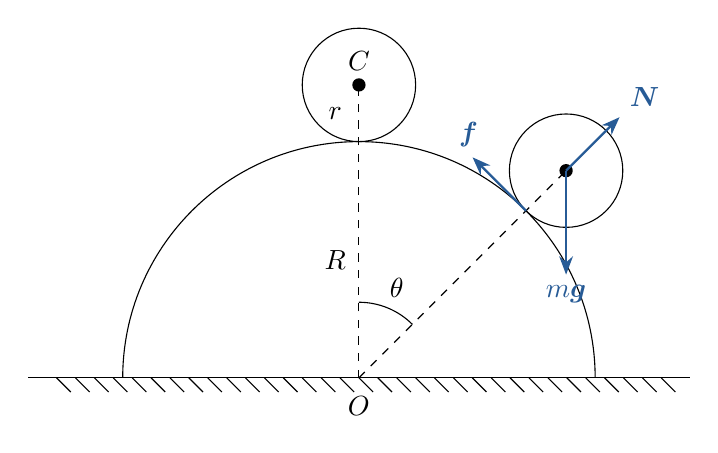
\begin{tikzpicture}[>=Stealth,scale=1.2]
    % 预定义深蓝色（与文档主题色统一）
    \definecolor{mainblue}{RGB}{39,91,150}
    
    % 几何参数
    \def\R{2.5}       % 大圆柱半径
    \def\r{0.6}       % 小球半径
    \def\alpha{45}    % 仅控制小球绘图位置，标注始终为θ
    \def\arrowLen{0.8}% 基础力箭头长度

    % 地面与斜线纹理（保持黑色）
    \draw (-3.5,0) -- (3.5,0);
    \foreach \x in {-3.2,-3.0,...,3.2} \draw (\x,0)--(\x+0.15,-0.15);

    % 固定大圆柱上半部分（保持黑色）
    \draw (-\R,0) arc[start angle=180,end angle=0,radius=\R];

    % 初始位置O-C竖直虚线与标注（保持黑色）
    \draw[dashed] (0,0) -- (0, \R+\r);
    \node at (-0.25, \R/2) {$R$};
    \node at (-0.25, \R + \r/2) {$r$};

    % 初始位置（最高点）的小球 + 质心圆点（保持黑色）
    \draw (0,\R+\r) circle (\r);
    \fill (0,\R+\r) circle (2pt);
    \node at (0,\R+\r+0.25) {$C$};

    % θ角位置的小球 + 质心圆点（保持黑色）
    \coordinate (C) at ({(\R+\r)*sin(\alpha)}, {(\R+\r)*cos(\alpha)});
    \draw (C) circle (\r);
    \fill (C) circle (2pt);

    % OC连线与角度标注（保持黑色）
    \draw[dashed] (0,0) -- (C);
    \draw (0,0.8) arc[start angle=90,end angle={90-\alpha},radius=0.8];
    \node at (0.4,0.95) {$\theta$};

    % 受力分析（箭头+标注全改为深蓝色）
    \coordinate (tangent) at ({\R*sin(\alpha)}, {\R*cos(\alpha)});
    % 重力mg
    \draw[->,thick,mainblue] (C) -- ++(0,-1.1) node[below,mainblue] {$m\boldsymbol{g}$};
    % 支持力N
    \draw[->,thick,mainblue] (C) -- ++({\arrowLen*sin(\alpha)}, {\arrowLen*cos(\alpha)}) node[above right,mainblue] {$\boldsymbol{N}$};
    % 静摩擦力f
    \draw[->,thick,mainblue] (tangent) -- ++({-\arrowLen*cos(\alpha)}, {\arrowLen*sin(\alpha)}) 
        node[above left, yshift=-0cm, xshift=0.2cm,mainblue] {$\boldsymbol{f}$};

    % 原点标注（保持黑色）
    \node at (0,-0.3) {$O$};
\end{tikzpicture}
\end{center}
\end{problemBox}

\section*{详细解法}
本题中我们需要找到静摩擦因数的最小值，这是因为当静摩擦因数过小时，最大静摩擦力过小，不能为小球提供足够力矩。因此我们需要先确定摩擦力大小与角度$\theta$的关系，保证$\theta = 45 ^{\circ}$时所需的静摩擦力依旧足以满足在圆柱表面纯滚动的要求。
\subsection*{1. 运动分析与坐标选取}
取地面为惯性参考系。 $OC$ 与竖直向上方向的夹角为 $\theta$，小球质心 $C$ 到固定圆柱面中心 $O$ 的距离为 $R+r$。  
质心 $C$ 的轨迹是以 $O$ 为圆心、半径为 $R+r$ 的圆弧。我们将尝试用 $\theta$ 作为自变量表示未知量。

\noindent 质心速度  
\[
v = (R+r)\dot{\theta},
\]
切向加速度  
\[
a_t = (R+r)\ddot{\theta},
\]
法向加速度  
\[
a_n = (R+r)\dot{\theta}^2 .
\]
纯滚动条件：设 $\phi$ 是小球自转角，顺时针为正，接触点速度为零，即 $v - r\dot{\phi} = 0$，故 $\dot{\phi} = v/r = (R+r)\dot{\theta}/r$，求导得  
\[
 \ddot{\phi} = \frac{R+r}{r}\,\ddot{\theta}.
\]
\subsection*{2. 受力分析}
小球受力：重力 $mg$（竖直向下），支持力 $N$（沿 $OC$ 方向背离 $O$），静摩擦力 $f$（沿切线方向，设为与下滑趋势相反的方向，即沿 $\theta$ 减小的切向）。  
受力方向已在题图中标出。

\subsection*{3. 列出动力学方程}
以 $O$ 为参考点的径向（指向 $O$ 为正）和横向（$\theta$ 增大方向为正）列质心平动的动力学方程：
\begin{numcases}{}
mg\cos\theta - N = m a_n = m(R+r)\dot{\theta}^2, \label{eq:1} \\[4pt]
mg\sin\theta - f = m a_t = m(R+r)\ddot{\theta}. \label{eq:2}
\end{numcases}
小球绕质心转动，转动惯量 $I_C = \dfrac{2}{5}mr^2$。静摩擦力对质心的力矩为 $f r$，角加速度 $\alpha = \ddot{\phi}$。转动方程：
\[
f r = I_C  \ddot{\phi} = \frac{2}{5}mr^2 \cdot \frac{R+r}{r}\,\ddot{\theta}
\]
即
\begin{equation}
f = \frac{2}{5}m(R+r)\ddot{\theta}. \label{eq:3}
\end{equation}
由于静摩擦力不做功，还有能量守恒方程：
\begin{equation}
\begin{aligned}
mg(R+r)(1-\cos\theta) &= \frac12 mv^2 + \frac12 I_C \dot{\phi}^2 \\
&= \frac12 m(R+r)^2\dot{\theta}^2 + \frac12\cdot\frac{2}{5}mr^2\cdot\left(\frac{R+r}{r}\dot{\theta}\right)^2 \\
&= \frac{7}{10}m(R+r)^2\dot{\theta}^2, \label{eq:4}
\end{aligned}
\end{equation}
一共有四个方程，而未知量包括$\dot{\theta}$, $\ddot{\theta}$, $N$ 和 $f$共四个，方程可解。
\subsection*{4. 求解未知量}
联立方程，解得
\[
\begin{cases}
\ddot{\theta} = \dfrac{5g\sin\theta}{7(R+r)} \\[8pt]
f = \dfrac{2}{7}mg\sin\theta \\[8pt]
\dot{\theta}^2 = \dfrac{10g(1-\cos\theta)}{7(R+r)} \\[8pt]
N = mg\left[\dfrac{17}{7}\cos\theta - \dfrac{10}{7}\right]
\end{cases}
\]
在 $\theta \le 45^\circ$ 范围内支持力N不是负数，所以在题给条件下不会出现球和圆柱分离的情况。
\subsection*{5. 纯滚动条件与 $\mu$ 的最小值}
保证不滑动，静摩擦力须满足 $f \le \mu N$，即
\[
\frac{2}{7}mg\sin\theta \le \mu \cdot mg\left(\frac{17}{7}\cos\theta - \frac{10}{7}\right),
\]
在 $\theta \le 45^\circ$ 范围内， $17\cos\theta-10 >0$，故可以移项得到
\[
\mu \ge \frac{2\sin\theta}{17\cos\theta - 10}.
\]
右端函数对 $\theta$ 单调递增，因此最大值在 $\theta = 45^\circ$ 处取得，为$\dfrac{34+20\sqrt2}{89}$，所以
\[
\boxed{\mu_{\min} = \frac{34+20\sqrt{2}}{89} \approx 0.70}
\]
因此，为保证在 $\theta \le 45^\circ$ 范围内小球始终做纯滚动，静摩擦因数至少应取此值。

\section*{技巧与知识点}
\begin{tipBox}
\begin{enumerate}
  \item \textbf{纯滚动与有滑动的本质区别：}
  纯滚动时接触点速度为零，可列出 $v = r\omega$ 及其导数形式的约束，但 \textbf{没有} $f = \mu N$ 的关系，此时静摩擦力是未知力，由动力学方程解出；一旦滑动，$f = \mu N$ 成立，但运动学约束消失，需根据滑动方向确定摩擦力方向。
  \item \textbf{未知量与方程个数校验：}
  在本题中，共列出平动、转动、能量守恒及纯滚动约束四个方程，对应 $\dot{\theta}$、$\ddot{\theta}$、$N$、$f$ 四个未知量，方程组封闭。解题时养成先统计未知量与方程数的习惯，可避免盲目联立。
  \item \textbf{静摩擦力方向的假定：}
  通常先假设静摩擦力与相对滑动趋势方向相反。若解出正值，假设正确；若为负值，表明实际方向相反，但不影响大小。本题中 $f$ 表达式为正，说明方向与所设一致。
  \item \textbf{转动方程的参考点选择：}
  对于刚体平面运动，转动方程通常对质心列出。
  \item \textbf{能量法的使用条件：}
  纯滚动中静摩擦力作用点瞬时速度为零，不做功，只有重力做功，因此机械能守恒。\textbf{若存在滑动摩擦力，则机械能不守恒}，一般不能直接使用能量方程。
\end{enumerate}
\end{tipBox}

\section*{复习建议}
刚体平面运动是本章重点，同时包括平动和定轴转动。处理滚动与摩擦问题时建议：
\begin{enumerate}
  \item 熟练掌握纯滚动约束的两种表达形式（速度形式和加速度形式），并能与平动、转动方程灵活联立。
  \item 练习“纯滚动”与“又滚又滑”两种运动的题目，体会方程结构的变化。
  \item 能量守恒只适用于纯滚动且无其他非保守力做功的情形。
  \item 注意静摩擦力方向一定要根据相对运动趋势判断，不能一概认为与运动方向相反。
  \item 临界问题通常归结为求某个比值的最值，善于利用函数单调性或导数分析，减少计算量。
  \item 养成“先看未知数个数，再数独立方程个数”的习惯，确保方程组可解后再动手代入消元，避免混乱。
\end{enumerate}

\end{document}